\documentclass{beamer}
\usetheme[pageofpages=of,% String used between the current page and the
                         % total page count.
          bullet=circle,% Use circles instead of squares for bullets.
          titleline=true,% Show a line below the frame title.
          alternativetitlepage=true,% Use the fancy title page.
       %   titlepagelogo=logo-polito,% Logo for the first page.
       %   watermark=watermark-polito,% Watermark used in every page.
       %   watermarkheight=100px,% Height of the watermark.
       %   watermarkheightmult=4,% The watermark image is 4 times bigger
                                % than watermarkheight.
          ]{Torino}

\setbeamertemplate{footline}{
  \begin{beamercolorbox}[wd=\paperwidth,ht=1ex,dp=1ex]{footline}
    \vspace{5pt} \hspace{1em} \insertframenumber/\inserttotalframenumber
  \end{beamercolorbox}
}

\author{Brendon J. Brewer}
\title{STATS 331 -- Introduction to Bayesian Statistics}
\institute{The University of Auckland}
\date{}


\linespread{1.3}
\usepackage{minted}
\usepackage[utf8]{inputenc}
\usepackage{dsfont}
\newcommand{\given}{\,|\,}
\newcommand{\balpha}{\boldsymbol{\alpha}}
\newcommand{\bmu}{\boldsymbol{\mu}}


\begin{document}

\frame{\titlepage}

\begin{frame}
\centering
\Large
Sports Prediction

\begin{center}
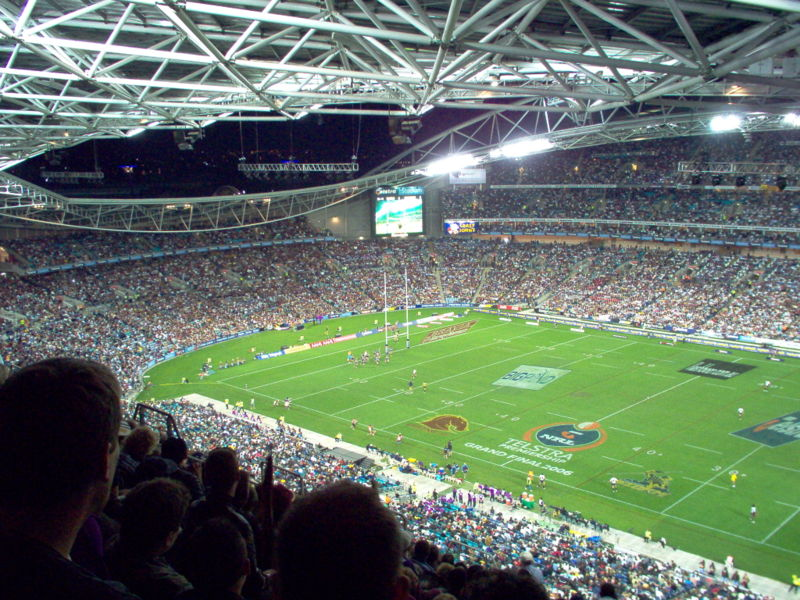
\includegraphics[width=0.6\textwidth]{images/football.jpg}

Credit: MDM, Wikimedia Commons
\end{center}

\end{frame}


\begin{frame}
\frametitle{Motivation}

\begin{itemize}
\item This is a `fun'\footnote{Your mileage may vary.}
lecture where each year I try to predict the NRL
(Rugby League tournament based in Australia) grand final result using Bayesian
statistics. \pause
\item It is somewhat related to logistic regression.\pause
\item The model will start off relatively simple, but will eventually
become a hierarchical model.
\end{itemize}
\end{frame}

\begin{frame}
\frametitle{NRL}

\begin{itemize}
\item The NRL is the (Australian) National Rugby League tournament (it also
includes the New Zealand Warriors).\pause
\item There are 17 teams in the competition.\pause
\item The grand final will be played on Sunday, between the teams:
TBD.
\end{itemize}
\end{frame}


\begin{frame}
\frametitle{The Data}
To predict the grand final result, we will use the data for who won every match
so far this season. We will fit a model with parameters describing the ability
of each team, and then do prediction in the usual way, in JAGS.\\[0.5em]\pause

I asked ChatGPT to write a little script to download this year's match results
from the web, and it succeeded!
\end{frame}


\begin{frame}[fragile]
\frametitle{The Data}

\begin{minted}{r}
> data = read.csv("nrl_2025_results.csv")
> head(data)
  home_team away_team home_score away_score home_team_win
1         1         2         30          8             1
2         3         4         28         22             1
3         5         6         14         50             0
4         7         8          8         10             0
5         9        10         16         14             1
6        11        12         20         28             0
\end{minted}

\end{frame}


\begin{frame}[fragile]
\frametitle{The Data}
For simplicity, we will only make use of the columns
\mintinline{r}{home_team} (the identity of the home team),
\mintinline{r}{away_team} (the identity of the away team),
and \mintinline{r}{home_team_win} (whether or not the home team won the match).
So we are throwing away information about
the scores and just looking at the winner of each match.

\end{frame}

\end{document}

